%% This is an example second chapter.  You should put chapter/appendix that you
%% write into a separate file, and add a line \include{yourfilename} to
%% main.tex, where `yourfilename.tex' is the name of the chapter/appendix file.
%% You can process specific files by typing their names in at the 
%% \files=
%% prompt when you run the file main.tex through LaTeX.
\chapter{Evaluating out-of-the-box BERT}

The poor performance of BERT$_{\mathrm{CoLA}}$ may have understandably raised many of the concerns we expressed in Section \ref{section:kol} regarding the strength of the conclusions that can be drawn from using a probing approach.  As it stands now, the results observed in Sections \ref{section:2.5.1} and \ref{section:2.5.2} suggest that the additional performance afforded by BERT$_{\mathrm{CoLA}}$ over a trigram model is due to the extra machinery relying on a collection of spurious correlations that provide good I.I.D. test set performance.

In order to verify the validity of this interpretation, we conduct one final case study.  Having seen how the ADC works as a function of $\delta$ and having compared it to the BLiMP criterion, we now apply it directly to the out-of-the-box versions of the BERT models (BERT$_{\mathrm{MLM}}$) studied in Chapter \ref{chapter:chapter2}.  This addresses what we see as two critical weak points in our analyses thus far.  The first is that of the instability during the fine-tuning phase observed in Section \ref{section:bert_instability}; there exists the possibility that there is a particular seed in which each BERT$_{\mathrm{CoLA}}$ model performs much better or much worse on the ADC.  The second is that we have no control over what information is being introduced into the system with CoLA.  Although we were clear about our expectations for BERT$_{\mathrm{CoLA}}$ and their basis in Section \ref{section:2.1}, we hope that by removing CoLA from the analysis pipeline, we address concerns regarding the lack of gradience in BERT$_{\mathrm{CoLA}}$'s output, as formulated in Equation \ref{eqn:bert_gradient_cola_output}.

\section{BERT Masked Language Modeling}
The pre-trained BERT models this thesis has been using in its analyses are the publicly available pre-trained model checkpoints originally published by Devlin et al. 2018.  The models were pre-trained using two tasks: Masked Language Modeling (MLM) and Next Sentence Prediction (NSP).  For these analyses, we will focus on MLM, a variant of the Cloze task (Taylor, 1953).  MLM involves randomly masking approximately 15\% of the subword tokens provided to the BERT model as input during training, with some variation in order to achieve robustness in later fine-tuning stages.  The model is then asked to predict the original token behind the mask by feeding the final hidden vector directly into a softmax ouptut layer with an output node for each item in the model's vocabulary.  The weight update is calculated afterward using cross entropy loss (Devlin et al. 2018).  

Because MLM is one of the tasks used to pre-train BERT in the first place, we use it to test the models in their out-of-the-box state.  By masking each token in a sentence $s_i$ sequentially and recovering the log likelihood of the original token, we are able to calculate a \textit{pseudo-log-likelihood} (PLL) score for the sentence.  Salazar et al. 2020 have shown that BERT's PLL scores are able to outperform GPT-2 on the BLiMP Criterion, as well as other natural language benchmarks.  They attribute this success to the PLL's unsupervised expression of linguistic acceptability without left-to-right bias (Salazar et al. 2020); BERT is better able to leverage the entire left and right context of each masked token in order to calculate original token's likelihood.  This altogether strongly favors PLL scores as the ideal metric to test the out-of-the-box BERT models with the ADC.

To express the concept of the PLL metric more formally, suppose we want to get the PLL score of the sentence \textit{Colorless green ideas sleep furiously} $s_i$ from BERT$_{\mathrm{MLM}}$.  For each word $w_j$ in the sentence $s_i$, we first replace $w_j$ using a \texttt{[MASK]} token, and then apply the softmax function defined in Equation \ref{eqn:softmax} directly on the encoded output $h_{i,j}$ of BERT$_{\mathrm{MLM}}$'s hidden layers, written below.
\begin{equation}
    P(w_j|h_{i,j}) = \mathrm{softmax}(h_{i,j})
    \label{eqn:mlm_token_prob_a}
\end{equation}
We can rewrite the probability of the token $w_j$ given the hidden vector $h_{i,j}$ as the probability of the token given its entire left and right context, the principal advantage of the MLM approach:
\begin{equation}
    P(w_j|w_0,...,w_{j-1},w_{j+1},...w_n)) = \mathrm{softmax}(h_{i,j})
    \label{eqn:mlm_token_prob_b}
\end{equation}
And now this final form can be used by Equation \ref{eqn:pseudo_log_likelihood}, which sums over the MLM log probabilities of each of the tokens to produce the \textit{pseudo log-likelihood}, PLL($s_i$).

\section{Correlations with human judgements}
Before applying the BLiMP Criterion and the ADC, it seems appropriate to carry out a pilot analysis by calculating the PCCs between the three BERT$_{\mathrm{MLM}}$ models and the human judgements when using the models' PLL scores for individual sentences in the LI-Adger datatset.  We present in Figure \ref{fig:bert_acc_pll_correlation_matrix} an updated correlation matrix containing the PCCs for the new PLL scores as well as the BERT$_{\mathrm{CoLA}}$ acceptability outputs presented in Figure \ref{fig:bert_acc_pll_correlation_matrix}.

\begin{figure}[h]
    %\centering
    \makebox[\textwidth][c]{
        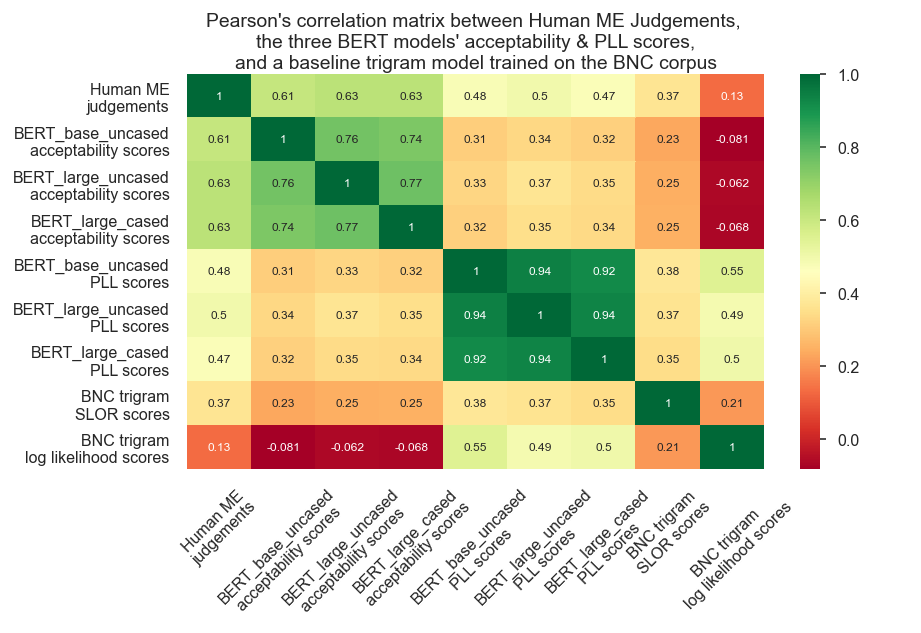
\includegraphics[scale=0.5]{templates/figures/bert_acc_pll_correlation_matrix.png}
    }
    \caption[PCC matrix between human judgements, BERT acceptability \newline \& PLL scores, and a trigram model]{PCC matrix between human judgements, BERT$_{\mathrm{CoLA}}$ acceptability scores, \& BERT$_{\mathrm{MLM}}$ PLL scores from all three BERT models.  In addition we add the SLOR and log likelihood scores of a trigram model trained on the British National Corpus by Sprouse et al. 2018 for additional reference.  All correlations shown have a $p$ < 0.0001.}
    \label{fig:bert_acc_pll_correlation_matrix}
\end{figure}


Additionally, we update our correlation graph from Figure \ref{fig:bert_acc_correlation_plot} in order to observe how the PLL scores may account for the full range of acceptability on an individual sentence level.

\begin{figure}[h!]
    %\centering
    \makebox[\textwidth][c]{
        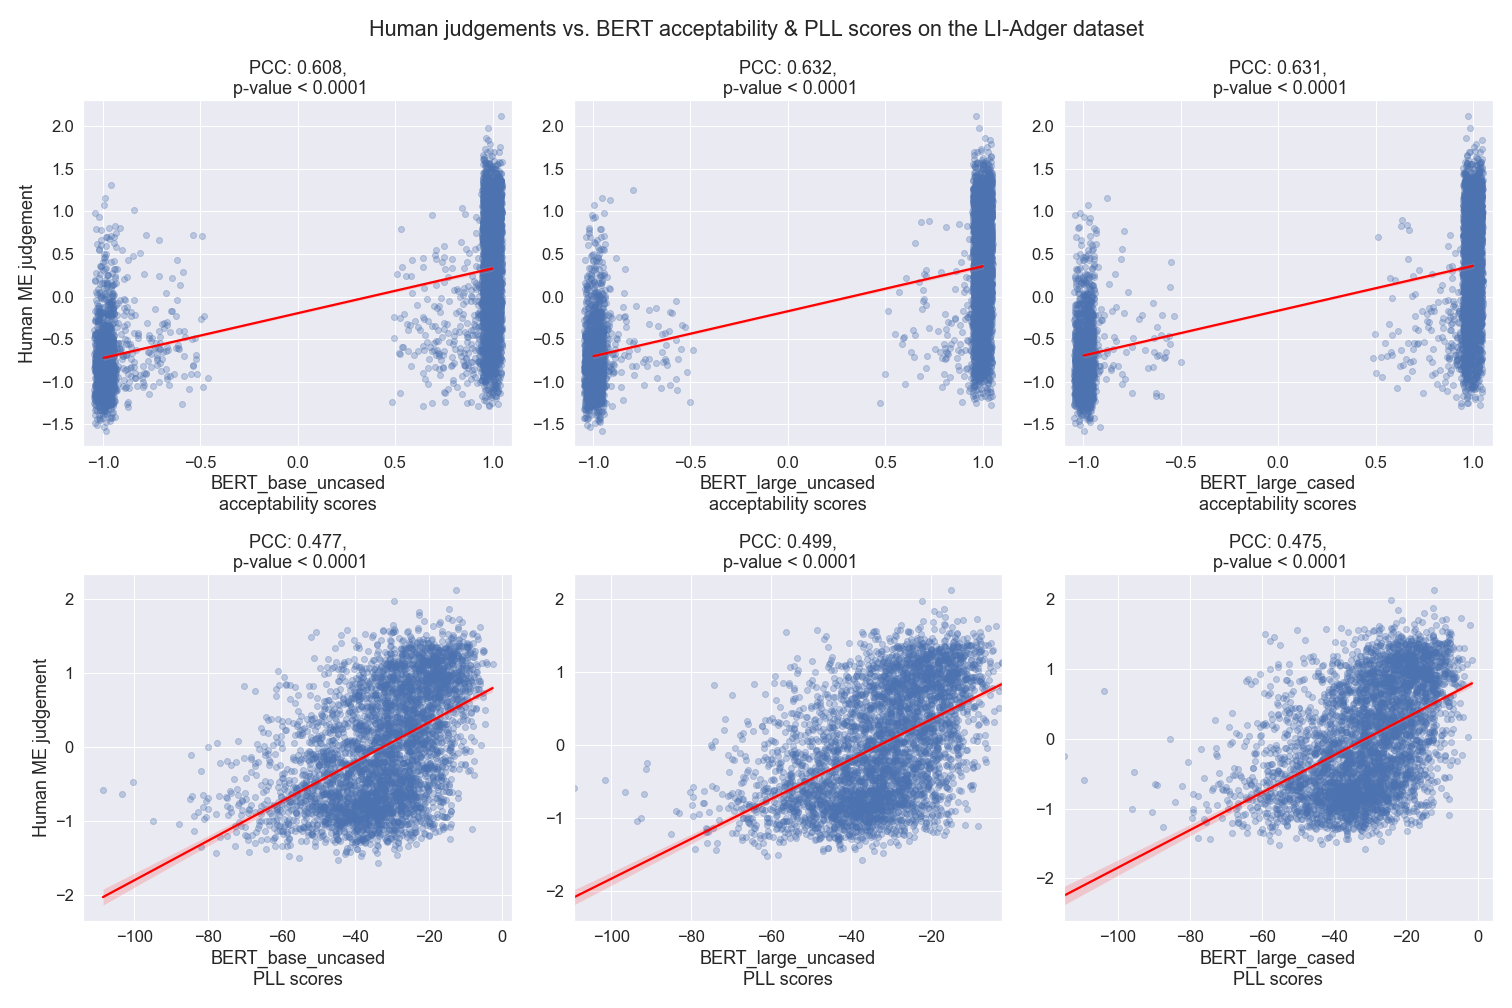
\includegraphics[scale=0.3]{templates/figures/bert_acc_pll_correlation_plot.png}
    }
    \caption[Human judgements vs. BERT acceptability \& PLL scores \newline on LI-Adger dataset]{Scatterplot of human judgements (y-axis) vs. BERT$_{\mathrm{CoLA}}$ acceptability scores, \& BERT$_{\mathrm{MLM}}$ PLL scores from all three BERT models for each sentence in the LI-Adger dataset with best-fit line in red.  We add a jitter of 0.05 along the x-axis and lower the alpha to 0.3 to highlight the density of the points.}
    \label{fig:bert_acc_pll_correlation_plot}
\end{figure}
\clearpage
If previous examples are on the mark, the fact that the PCCs for the BERT$_\mathrm{MLM}$ PLL scores are, on average, around 0.15 points lower than the corresponding BERT$_\mathrm{CoLA}$ acceptability scores is not indicative of performance on the ADC.  At least now with the PLL scores, the sentences truly seem to line up on a gradient scale, and one that appears to roughly track the best-fit line much better than the acceptability scores.  The next step is to calculate the PCCs for the Z-score transformed PLL deltas and add them to the correlation matrix in Figure \ref{fig:bert_acc_delta_correlation_matrix} in order to see how the PCCs change according to the more gradient metric.  We present in Figure \ref{fig:bert_acc_pll_delta_correlation_matrix} the updated correlation matrix comparing the baseline trigram model, BERT$_{\mathrm{CoLA}}$ acceptability delta scores and the newly calculated BERT$_{\mathrm{MLM}}$ PLL delta scores.

\begin{figure}[h]
    %\centering
    \makebox[\textwidth][c]{
        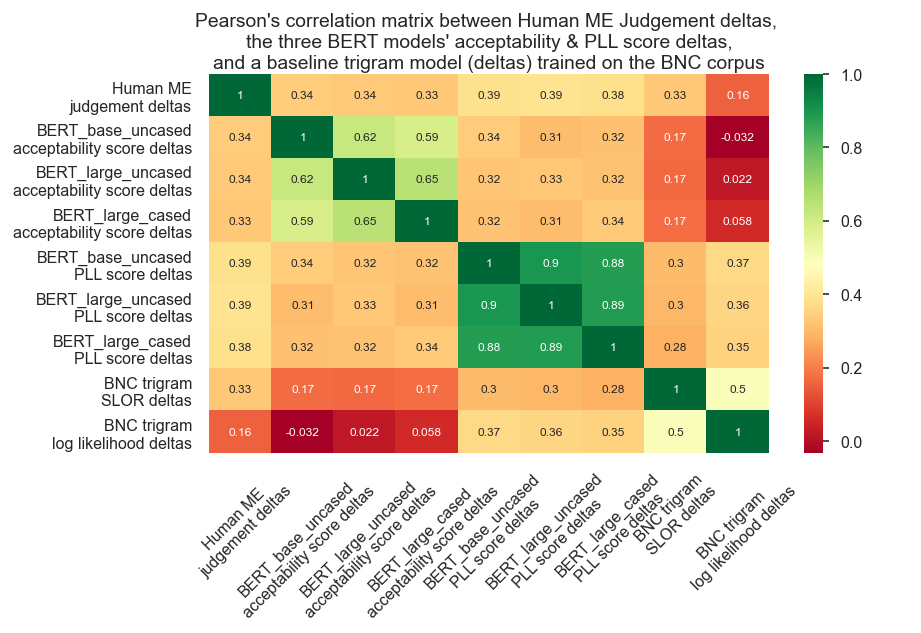
\includegraphics[scale=0.5]{templates/figures/bert_acc_pll_delta_correlation_matrix.png}
    }
    \caption[PCC matrix between human judgements, BERT$_{\mathrm{CoLA}}$,\newline BERT$_{\mathrm{MLM}}$, and a trigram model]{PCC matrix between human judgements and all three BERT$_{\mathrm{CoLA}}$ \& BERT$_{\mathrm{MLM}}$.  In addition we add the SLOR and log likelihood scores of a trigram model trained on the British National Corpus by Sprouse et al. 2018 for additional reference.  All correlations shown have a $p$ < 0.0001.}
    \label{fig:bert_acc_pll_delta_correlation_matrix}
\end{figure}

Encouragingly, we see a similar scenario to that of the trigram's SLOR score deltas and the three BERT$_{\mathrm{CoLA}}$s' acceptability score deltas discussed in Section \ref{section:2.5.1}.  Although the BERT$_{\mathrm{CoLA}}$s' acceptability scores at the individual sentence level obtain much higher PCCs with the human judgements on the LI-Adger dataset, that advantage disappears when calculating the PCCs between the human judgement deltas and the acceptability score deltas.  We see in Figure \ref{fig:bert_acc_pll_delta_correlation_matrix} that the PLL score deltas overtake the acceptability score deltas, although only by a small margin.  For completeness, we plot in Figure \ref{fig:bert_acc_pll_delta_correlation_plot} once more the correlation graphs in Figure \ref{fig:bert_acc_delta_correlation_plot} but adding the PLL score deltas to the comparison.
\begin{figure}[h]
    %\centering
    \makebox[\textwidth][c]{
        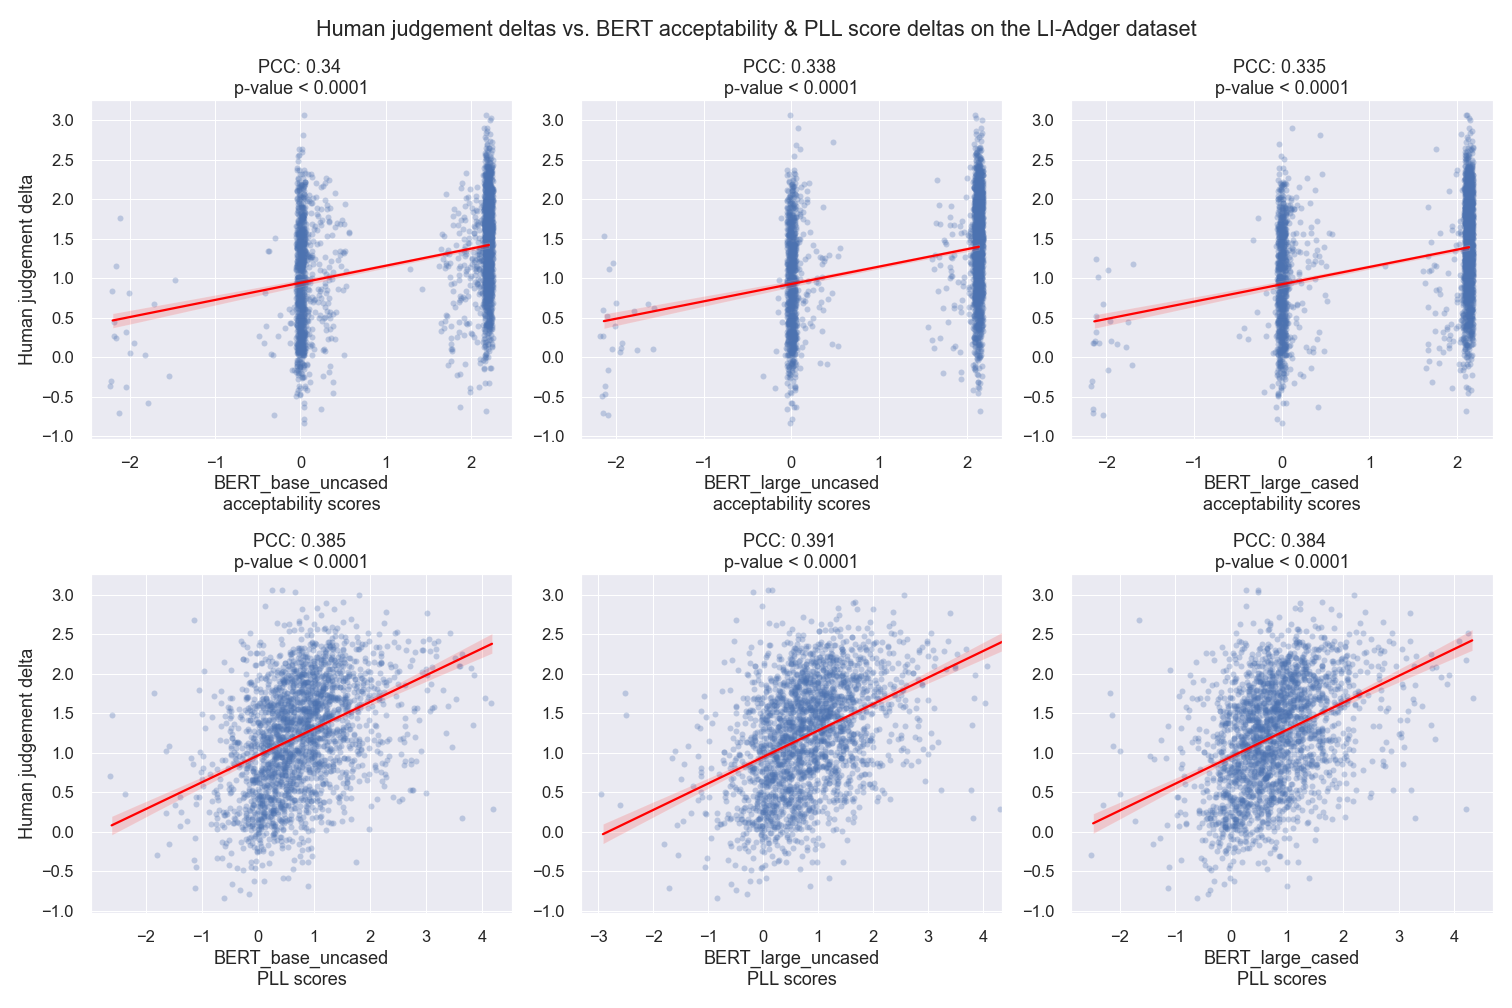
\includegraphics[scale=0.3]{templates/figures/bert_acc_pll_delta_correlation_plot.png}
    }
    \caption[Human judgements vs. BERT acceptability \& PLL scores \newline on LI-Adger minimal pairs]{Scatterplot of human judgement deltas (y-axis) vs. BERT$_{\mathrm{CoLA}}$ acceptability score delta \& BERT$_{\mathrm{MLM}}$ PLL delta for each minimal pair in the LI-Adger dataset with best-fit line in red.  We add a jitter of 0.05 along the x-axis and lower the alpha to 0.3 to highlight the density of the points.}
    \label{fig:bert_acc_pll_delta_correlation_plot}
\end{figure}

With all the preliminary correlations in place, we can set reasonable expectations for the BERT$_{\mathrm{MLM}}$ models' performance under the ADC using the PLL deltas.  We believe the gradience shown both at the sentence level PLL scores and the PLL deltas at the minimal pair level will yield better performance under the ADC at all three levels tested ($\delta=0.5$, $\delta=1.0$ and $\delta=5.0$).  How much better that performance is, remains to be seen.

\section{BERT says best 2 out of 3 (ADC round 2)}
Similar to Section \ref{section:2.5.2}, we apply the BLiMP Criterion and the ADC with $\delta=\{0.5, 1.0, 5.0\}$ in order to see how the ADC scales as it becomes less strict and generalizes to a form similar to the BLiMP Criterion.  We report the performance of the three BERT$_{\mathrm{MLM}}$ models using their PLL scores along with all the previously evaluated models in Table \ref{tab:table_15}.
\begin{table}[h]
    \centering
    \ra{1.3}
    \begin{tabular}{@{}lcccc@{}}
    \toprule
    \textbf{Model} & \textbf{BLiMP} & \textbf{ADC, $\delta=0.5$} & \textbf{ADC, $\delta=1.0$} & \textbf{ADC, $\delta=5.0$}  \\
    \midrule
    BERT$_{base-uncased; \mathrm{MLM}}$ & 0.852 & 0.364 & 0.631 & 0.849 \\
    BERT$_{large-uncased; \mathrm{MLM}}$ & 0.866 & 0.378 & 0.658 & 0.859 \\
    BERT$_{large-cased; \mathrm{MLM}}$ & 0.871 & 0.376 & 0.661 & 0.868 \\
    \midrule
    BERT$_{base-uncased; \mathrm{CoLA}}$ & 0.915 & 0.286 & 0.538 & 0.902 \\
    BERT$_{large-uncased; \mathrm{CoLA}}$ & 0.917 & 0.311 & 0.564 & 0.907 \\
    BERT$_{large-cased; \mathrm{CoLA}}$ & 0.936 & 0.307 & 0.561 & 0.925 \\
    \midrule
    trigram$_{SLOR}$ & 0.753 & 0.301 & 0.520 & 0.744\\
    trigram$_{log-prob}$ & 0.671 & 0.165 & 0.329 & 0.668 \\
    \bottomrule
    \end{tabular}
    \caption[BERT$_{\mathrm{MLM}}$, BERT$_{\mathrm{CoLA}}$, and trigram model scores\newline under BLiMP \& ADC]{Comparison between the models' BLiMP and ADC scores, using $\delta$=\{0.5, 1.0, 5.0\}. We include three BERT$_{\mathrm{MLM}}$ models, three BERT$_{\mathrm{CoLA}}$ models, as well as SLOR and log-likelihood scores from a trigram model trained on the British National Corpus by Sprouse et al. 2018}
    \label{tab:table_15}
\end{table}

Reassuringly, the higher PCCs shown in Figures \ref{fig:bert_acc_pll_delta_correlation_matrix} and \ref{fig:bert_acc_pll_delta_correlation_plot} by the BERT$_{\mathrm{MLM}}$ models' PLL output translate well to better performance than the BERT$_{\mathrm{CoLA}}$ models on the ADC for $\delta=0.5$ and $\delta=1.0$.  However, when the distance between the models' output deltas and the human judgement deltas (Equation \ref{eqn:acceptability_delta_criterion_b}) is no longer considered by the ADC ($\delta=5.0$), the BERT$_{\mathrm{CoLA}}$ models outperform the BERT$_{\mathrm{MLM}}$ models.  This is likely due to the lack of gradience in the BERT$_{\mathrm{CoLA}}$ models' acceptability output no longer being a determining factor in whether they evaluated a minimal pair correctly or not. This is presented in more detail below. First, as in Section \ref{section:2.5.2}, we inspect 4 minimal pairs where the BERT$_{\mathrm{MLM}}$ models meet the BLiMP Criterion but not the ADC with a $\delta=5.0$, shown in Table \ref{tab:table_16}.  

\begin{table}[h]
    \centering
    \ra{1.3}
    \begin{tabular}{@{}lcc@{}}
    \toprule
    \textbf{Minimal Pair} & Human & BERT$_{\mathrm{MLM}}$\\
    \textbf{Top}: Acceptable | \textbf{Bottom}: Unacceptable & judgement & PLL\\
    \toprule
    What is there a coupon for on the counter?  & 0.085185 & 0.731265 \\
    *What is a coupon for on the counter? & 0.134364 & 0.00874871 \\
    \midrule
   What the runners believe is that they will win the race. & -0.23705 &  1.44651 \\
    *What the runners believe is they will win the race. &  -0.1155 & 1.1792 \\
    \midrule
    I guessed he was married. & 0.111685 & 1.3683 \\
    *I guessed he is married.  &  0.588843	 & 0.753377 \\
    \midrule
    The announcer's introduction of Ted was humorous.  & 0.659471 & 0.52595 \\
    *The announcer's introduction of Ted's was humorous. & 0.748718 & 0.378315 \\
    \bottomrule
    \end{tabular}
    \caption[Four minimal pairs where BERT$_{\mathrm{MLM}}$ meets the BLiMP\newline Criterion but not the ADC with $\delta=5.0$]{Four minimal pairs where all 3 models BERT$_{\mathrm{MLM}}$ passed the BLiMP criterion but not the generalized ADC with $\delta=5.0$. We report the BERT$_{\mathrm{MLM}}$ PLL scores from BERT$_{\mathrm{MLM}_{\mathrm{large-cased}}}$. The human judgement and BERT$_{\mathrm{MLM}}$ PLL scores are already z-score transformed.}
    \label{tab:table_16}
\end{table}

Although the three BERT$_{\mathrm{MLM}}$ models failed to meet the ADC with $\delta=5.0$ in Table \ref{tab:table_16}, the reported PLL scores from BERT$_{\mathrm{MLM}_{\mathrm{large-cased}}}$ immediately show how BERT$_{\mathrm{MLM}}$'s PLL scores are much more gradient than the acceptability outputs from the BERT$_{\mathrm{CoLA}}$ models.  Let us inspect a few more example minimal pairs, but this time those where the BERT$_{\mathrm{MLM}}$ models met the ADC with $\delta=5.0$ but not the BLiMP Criterion, shown in Table \ref{tab:table_17}.

\begin{table}[h]
    \centering
    \ra{1.3}
    \begin{tabular}{@{}lcc@{}}
    \toprule
    \textbf{Minimal Pair} & Human & BERT$_{\mathrm{MLM}}$\\
    \textbf{Top}: Acceptable | \textbf{Bottom}: Unacceptable & judgement & PLL\\
    \toprule
    We proved Amelia to the manager to be responsible.  & -0.56008 & -1.77701 \\
    *We proved to the manager Amelia to be responsible. & -0.13864 & -1.26881 \\
    \midrule
    What did you give to whom? & 0.082244 & 0.899228 \\
    *To whom did you give what? & 0.289657 & 0.930362 \\
    \midrule
    There is likely to depart a train at midnight. & -0.53097 & -0.706574 \\
    *There is likely a train to depart at midnight.  &  0.177497 & 0.441587 \\
    \midrule
    Jenny would accurately have calculated the results. & 0.345683 & -1.90655 \\
    *Jenny accurately will calculate the results.  & 0.501494 & -0.458686 \\
    \bottomrule
    \end{tabular}
    \caption[Four minimal pairs where BERT$_{\mathrm{MLM}}$ meets the ADC\newline with $\delta=5.0$ but not the BLiMP Criterion]{Four minimal pairs where all 3 BERT$_{\mathrm{MLM}}$ models pass the generalized ADC with $\delta=5.0$ but not the BLiMP criterion. We report the BERT$_{\mathrm{MLM}}$ PLL scores from BERT$_{\mathrm{MLM}_{\mathrm{large-cased}}}$. The human judgement and BERT$_{\mathrm{MLM}}$ PLL scores are already z-score transformed.}
    \label{tab:table_17}
\end{table}

What all the example minimal pairs in Table \ref{tab:table_17} have in common is that the human judgements disagree with the expert labels.  Therefore, if we were to evaluate the human judgements themselves under the BLiMP Criterion, they would not pass either.  However, reading the second and third minimal pair in Table \ref{tab:table_17} highlights precisely why it is preferable to rely on human judgements before the expert labels: those two minimal pairs are very close in acceptability values, and in fact read almost the same to native speakers.  This additional resolution is lost when switching to categorical expert labels such as those required by BLiMP.  The BERT$_{\mathrm{MLM}}$ PLL scores agree in monotonicity with the human judgements too; that is, the three BERT$_{\mathrm{MLM}}$ models scored the unacceptable sentence in the minimal pair higher than the acceptable sentence, following the trend in the human judgements for the four examples in Table \ref{tab:table_17}.  Unfortunately, this is not a consistent trend.  For example, upon inspection of a few examples where the BERT$_{\mathrm{CoLA}}$ models meet the generalized ADC ($\delta=5.0$) but not the BERT$_{\mathrm{MLM}}$ models, we see the added gradience of the PLL scores alone is not enough.  The four examples in Table \ref{tab:table_18} show the BERT$_{\mathrm{CoLA}}$ models follow the monotonicity of the human judgements, whilst the BERT$_{\mathrm{MLM}}$ models flip which sentence is the more acceptable of the pair.  Under $\delta=5.0$, the lack of gradience no longer affects the BERT$_{\mathrm{CoLA}}$ models, thus allowing them to finally score higher than the BERT$_{\mathrm{MLM}}$ models, which they were unable to do for $\delta=0.5$ nor $\delta=1.0$.  However, there are cases where, even with $\delta=5.0$, BERT$_{\mathrm{MLM}}$ scores minimal pairs correctly that BERT$_{\mathrm{CoLA}}$ is unable to account for, show in Table \ref{tab:table_19}.

\begin{table}[h]
    \centering
    \ra{1.3}
    \begin{tabular}{@{}lccc@{}}
    \toprule
    \textbf{Minimal Pair}                                    & Human & BERT$_{\mathrm{CoLA}}$   & BERT$_{\mathrm{MLM}}$ \\
    \textbf{Top}: Acceptable | \textbf{Bottom}: Unacceptable & judgement & acceptability      & PLL\\
    \toprule
    The book was written truthfully.  & 1.30085 & 0.732642 & 1.00074 \\
    *The book writes truthfully. & -0.40842 & -1.40058 & 1.03895 \\
    \midrule
    It stormed suddenly. & 0.548385 & -1.39038 & 0.506643 \\
    *It suddenly stormed.    & 0.451832 &  -1.39582 & 0.785855 \\
    \midrule
    How few people were there at the rally? & 0.371244 & 0.732758 & 0.989334 \\
    *How few people there were at the rally? & -0.01639 & 0.732748 & 1.02265 \\
    \midrule
    The IRS denied Lilly her refund.  & 1.40233 & 0.732951 & -1.22485 \\
    *The IRS denied her refund to Lilly. & -0.47087 & 0.612725 & -0.966726 \\
    \bottomrule
    \end{tabular}
    \caption[Four minimal pairs where BERT$_{\mathrm{CoLA}}$ meets ADC \newline with $\delta=5.0$ but the BERT$_{\mathrm{MLM}}$ models do not]{Four minimal pairs where all BERT$_{\mathrm{CoLA}}$ models meet the ADC with $\delta=5.0$ but the BERT$_{\mathrm{MLM}}$ models do not. We report the scores from BERT$_{large-cased}$. The human judgement, acceptability, and PLL scores are already z-score transformed. }
    \label{tab:table_18}
\end{table}

\begin{table}[h]
    \centering
    \ra{1.3}
    \begin{tabular}{@{}lccc@{}}
    \toprule
    \textbf{Minimal Pair}                                    & Human & BERT$_{\mathrm{CoLA}}$   & BERT$_{\mathrm{MLM}}$\\
    \textbf{Top}: Acceptable | \textbf{Bottom}: Unacceptable & judgement & acceptability      & PLL\\
    \toprule
    Toby said to Sally to take care of herself.  & 0.188154 & -1.39838
 & 0.540271 \\
    *Toby said to Sally to take care of himself. & -0.488670 & 0.608852 & 0.348782 \\
    \midrule
    I predicted she was guilty.  & 0.703876 & 0.730575 & 0.615354 \\
    *I predicted she may be guilty.	 & 0.530117 &  0.732155 & 0.18414 \\
    \midrule
    The ice melted quickly on the table. & 1.459752	 & 0.729108 & 1.34043 \\
    *The ice quickly melted on the table. & 0.618948 & 0.730474 & 1.18234 \\
    \midrule
    A lawyer smarter than my brother...  & 0.596167 & 0.733196 & -0.188386 \\
    *A smarter lawyer than my brother... & 0.782106 & 0.733102 & 0.123958 \\
    \bottomrule
    \end{tabular}
    \caption[Four minimal pairs where BERT$_{\mathrm{MLM}}$ meets ADC\newline with $\delta=5.0$ but BERT$_{\mathrm{MLM}}$ does not]{Four minimal pairs where all BERT$_{\mathrm{MLM}}$ models meet the ADC with $\delta=5.0$ but not the BERT$_{\mathrm{CoLA}}$ models. We report the scores from BERT$_{large-cased}$. The human judgement, acceptability, and PLL scores are already z-score transformed. }
    \label{tab:table_19}
\end{table}
\clearpage
%\todo[inline]{Bob asks why using the surrounding context of the masked token is in principle similar to the ngram}

Our analyses of the BERT$_{\mathrm{MLM}}$ models continue by conducting the same trigram-overlap analyses we did with the BERT models fine-tuned using CoLA.  \textit{A priori} there likely is a much larger overlap between the trigram model's SLOR predictions and BERT$_{\mathrm{MLM}}$'s PLL predictions by the very nature of the MLM procedure.  BERT$_{\mathrm{MLM}}$ uses the surrounding context of a masked token to predict a probability distribution $P(w_j|w_0,...,w_{j-1},w_{j+1},...w_n)$ (Equation \ref{eqn:mlm_token_prob_b}) for each token in a given sequence of words $s_i$.  This is, in principle, similar to a trigram using the preceding context of a word to predict its likelihood $P(w_j|w_{j-3},w_{j-2},w_{j-1})$.  We say \textit{in principle} because the MLM and $N$-gram outputs and training regimes can be framed in terms of predicting individual tokens given their context, with the caveat that the trigram is severely handicapped in terms of the machinery it has at its disposal.  However, BERT$_{\mathrm{CoLA}}$ outputs a probability distribution over a finite set of categorical labels when given the entire sequence $s_i$ as input, so it is much farther removed from the computations a trigram performs relative to BERT$_{\mathrm{MLM}}$.  We assess the extent of this similarity by calculating the ADC for $\delta=0.5$ and $\delta=1.0$ once again.  Then for each value of $\delta$, we create a new dataset by subtracting the minimal pairs from LI-Adger dataset that were correctly predicted by the trigram's SLOR scores.  We finalize by recalculating the BERT$_{\mathrm{MLM}}$ models' ADC scores using the reduced datasets.  The results for the procedure are presented in Table \ref{tab:table_20}.

%\begin{table}[h]
    %\centering
    %\ra{1.3}
    %\begin{tabular}{@{}cccc@{}}
    %\toprule
    %\textbf{Model} & \textbf{ADC, $\delta=0.5$} & \textbf{ADC, %$\delta=0.5$} & \textbf{Total} \\
                   %& \textbf{original}          & \textbf{sans trigram}      & \textbf{overlap}\\
    %\midrule
    %BERT$_{base-uncased; \mathrm{MLM}}$ & 0.364 & 0.323 & 13.87\% \\
    %BERT$_{large-uncased; \mathrm{MLM}}$ & 0.378 & 0.333 & 14.50\% \\
    %BERT$_{large-cased; \mathrm{MLM}}$ & 0.376 & 0.335 & 14.21\% \\
    %\bottomrule
    %\end{tabular}
    %\caption[MLM-objective BERT models' ADC with $\delta=0.5$ scores sans easy min pairs]{MLM-objective BERT models' performance on the ADC with $\delta=0.5$ before and after removing all minimal pairs for which the ADC Criterion was met by the trigram baseline model trained on the BNC corpus. The third column is the percentage of BERT's passing minimal pairs that the trigram baseline also passed.}
    %\label{tab:xxxxx}
%\end{table}

%\begin{table}[h]
    %\centering
    %\ra{1.3}
    %\begin{tabular}{@{}cccc@{}}
    %\toprule
    %\textbf{Model} & \textbf{ADC, $\delta=1.0$} & \textbf{ADC, %$\delta=0.5$} & \textbf{Total} \\
                   %& \textbf{original}          & \textbf{sans trigram}      & \textbf{overlap}\\
    %\midrule
    %BERT$_{base-uncased; \mathrm{MLM}}$ & 0.631 & 0.553 & 36.58\% \\
    %BERT$_{large-uncased; \mathrm{MLM}}$ & 0.658 & 0.586 & 37.51\% \\
    %BERT$_{large-cased; \mathrm{MLM}}$ & 0.661 & 0.589 & 37.80\% \\
    %\bottomrule
    %\end{tabular}
    %\caption[MLM-objective BERT models' ADC with $\delta=1.0$ scores sans easy min pairs]{MLM-objective BERT models' performance on the ADC with $\delta=1.0$ before and after removing all minimal pairs for which the ADC Criterion was met by the trigram baseline model trained on the BNC corpus. The third column is the percentage of minimal pairs that both the BERT model and the trigram baseline pass.}
    %\label{tab:xxxxxxx}
%\end{table}

\begin{table}[h!]
    \centering
    \ra{1.3}
    \begin{tabular}{@{}lcccccc@{}}
    \toprule
    \textbf{Model} & \multicolumn{3}{c}{\textbf{ADC, $\delta=0.5$}} &  \multicolumn{3}{c}{\textbf{ADC, $\delta=1.0$}} \\
    \cmidrule{2-3} \cmidrule{4-7}
    \textbf{BERT}$_\mathrm{MLM}$ & \textbf{Original} & \textbf{Reduced} & \textbf{Overlap} & \textbf{Original} & \textbf{Reduced} & \textbf{Overlap} \\
    \midrule
    base-uncased & 0.364 & 0.323 & 13.87\% & 0.631 & 0.553 & 36.58\%\\
    large-uncased & 0.378 & 0.333 & 14.50\% & 0.658 & 0.586 & 37.51\%\\
    large-cased & 0.376 & 0.335 & 14.21\% &  0.661 & 0.589 & 37.80\% \\
    \bottomrule
    \end{tabular}
    \caption[BERT$_{\mathrm{MLM}}$ ADC with $\delta=$\{0.5,1.0\} scores\newline sans easy min pairs]{BERT$_{\mathrm{MLM}}$ models' performance on the ADC with $\delta$={0,5,1.0} before (Original) and after (Reduced) removing all minimal pairs for which the ADC Criterion was met by the trigram baseline model trained on the BNC corpus. The Overlap columns display the percentage of minimal pairs that both the BERT$_{\mathrm{MLM}}$ model and the trigram baseline pass.}
    \label{tab:table_20}
\end{table}

A difference that becomes immediately apparent is the drop in total performance across the board for all three BERT$_{\mathrm{MLM}}$ models both for $\delta=0.5$ and $\delta=1.0$ once the minimal pairs correctly scored by the trigram are removed from the dataset.  Unsurprisingly, the percentage of the minimal pairs scored correctly by both BERT$_{\mathrm{MLM}}$ and the trigram SLOR model correctly is on average 14.2\% for $\delta=0.5$ (up from 8.8\% with BERT$_{\mathrm{CoLA}}$) and 37.3\% for $\delta=1.0$ (up from 28.8\% with BERT$_{\mathrm{CoLA}}$).

Finally, this brings us to the question posed at the end of Chapter \ref{chapter:chapter2}: What is lost (or gained) in terms of performance under the ADC by switching from  BERT$_{\mathrm{CoLA}}$ acceptability scores to BERT$_{\mathrm{MLM}}$ PLL scores?  We present in Table \ref{tab:table_22} the performance of BERT$_{\mathrm{MLM}}$ under the ADC as shown previously, but add an additional column containing the percentage of overlap between BERT$_{\mathrm{MLM}}$ and BERT$_{\mathrm{CoLA}}$, i.e. what percentage of the minimal pairs in the LI-Adger dataset was classified correctly by both BERT models.  We carry out this calculation for $\delta=0.5$ and $\delta=1.0$ as with the trigrams assessment because these are where ADC enforces the gradient aspect of the minimal pairs, not just their monotonicity.

\begin{table}[h!]
    \centering
    \ra{1.3}
    \begin{tabular}{@{}lcccc@{}}
    \toprule
    \textbf{Model} & \multicolumn{2}{c}{\textbf{ADC, $\delta=0.5$}} &  \multicolumn{2}{c}{\textbf{ADC, $\delta=1.0$}} \\
    \cmidrule{2-3} \cmidrule{4-5}
    \textbf{BERT}$_{\mathrm{MLM}}$ & \textbf{Score} & \textbf{Overlap} & \textbf{Score} & \textbf{Overlap}  \\
    \midrule
    base-uncased & 0.364 & 9.05\% & 0.631 & 34.25\% \\
    large-uncased & 0.378 & 9.73\% & 0.658 & 37.29\% \\
    large-cased & 0.376 & 9.89\% & 0.661 & 37.04\% \\
%    \midrule
%    BERT$_{base-uncased; \mathrm{CoLA}}$ & 0.286 & 9.05\% & 0.538 & 34.25\% \\
%    BERT$_{large-uncased; \mathrm{CoLA}}$ & 0.311 & 9.73\% & 0.564 & 37.29\% \\
%    BERT$_{large-cased; \mathrm{CoLA}}$ & 0.307 & 9.89\% & 0.561 & 37.04\% \\
    \bottomrule
    \end{tabular}
    \caption[Overlap between BERT$_{\mathrm{MLM}}$ and BERT$_{\mathrm{CoLA}}$ under the ADC]{The percentage of minimal pairs that both BERT$_{\mathrm{MLM}}$ and BERT$_{\mathrm{CoLA}}$ passed, as well as the ADC scores with $\delta$=\{0.5, 1.0\} of the BERT$_{\mathrm{MLM}}$ models for reference.}
    \label{tab:table_22}
\end{table}

The overlap between BERT$_{\mathrm{MLM}}$ and BERT$_{\mathrm{CoLA}}$, although substantial, only accounts for roughly one third of the minimal pairs either of the two models scored correctly under the stricter $\delta=0.5$ measure.  Relaxing the ADC to $\delta=1.0$ allows the overlap between the two models to account for roughly half of the minimal pairs they each scored correctly.  However, this supports the interpretation we set out to test at the beginning of this chapter: BERT$_{\mathrm{MLM}}$ and BERT$_{\mathrm{CoLA}}$ behave almost completely differently, even demonstrating different KoL despite relying on the same pretrained BERT model.  Training an additional classifier on top of BERT, as we did with CoLA, further obfuscates any information to be gained from conducting an input-output analysis on the model.

%\section{A successful maiden voyage for ADC}


%Using the BERT$_{\mathrm{CoLA}}$ and 


%The lack of gradience demonstrated by the BERT models fine-tuned using the CoLA training set provided the optimal 





